\documentclass{article}
\usepackage{tikz, comment}
\usepackage{pifont}
\usepackage{fontspec, pgfplots}
\usetikzlibrary{arrows, decorations.markings, decorations.pathreplacing}
\begin{comment}
:Title: Not defined yet
:Tags: absolute value rules;properties of equality, equation rules;set;trichotomy;proper subset
:Prob: 0.5317;0.5167;0.5119;0.5069;0.4851
:Author: Prof.Hu Ji-shan, HKUST
:Slug: No name yet

Description Here.........
\end{comment}
\begin{document}\centering 

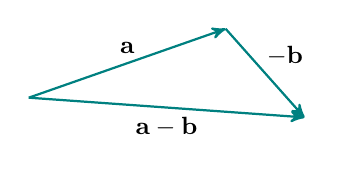
\begin{tikzpicture}[>=latex,xscale=.5*5, yscale=.5*5][font=\sf\small] 

\draw[teal, thick, ->, >=stealth'] (0, 0) -- (1, 0.35)node[black, above, midway, pos=0.5, xshift=0, yshift=0, scale=1]{$\bf a$}; %a

\begin{scope}[xshift=1cm,yshift=0.35cm]
\draw[teal, thick, ->, >=stealth'] (0, 0) -- (0.4, -0.45)node[black, right, midway, pos=0.4, xshift=0, yshift=3, scale=1]{$\bf -b$}; %-b
\end{scope}

\draw[teal, thick, ->, >=stealth'] (0, 0) -- ({1+0.4}, {0.35-0.45})node[black, below, midway, pos=0.5, xshift=0, yshift=0, scale=1]{$\bf a-b$};

\end{tikzpicture}
\end{document}